% !TEX root = BA-Bericht.tex
\chapter{Einleitung}
\label{ch:Einleitung}
% TODO Allgemeine Einleitung in die Arbeit

Das Internet Protokoll (IP) ist eines der wichtigsten Grundsteine für das heutige Internet.
Dieses wurde jedoch damals unter nicht den gesichtspunkten wie Datenschutz, Privatsphäre und Sicherheit designt.
Es ging wohl eher darum, dass überhaupt ein Protokoll da war, um Nachrichten in einem Netzwerk verschicken von Knoten von Knoten weiterleiten zu können.
Mittlerweile gibt es jedoch verschiedene Anonymisierungsnetzwerke, welche in diesem Bereich Abhilfe schaffen könnten.
Eines davon nennt sich ''\glstext{i2p}'' (kurz \glsname{i2p}), welches in dieser Arbeit genauer untersucht wird.
Die Performanz von Anonymisierungsnetzwerken ist aber nie vergleichbar mit der Performanz des Internet Protokolls.
Denn einerseits verwenden auch diese das Internet Protokoll und andererseits gibt es verschiedene weitere Einschränkungen, falls Anonymität in einem Netzwerk geschaffen werden soll (siehe Abschnitt~\fullref{sec:anonymitytrilemma}). Für Benutzer lässt die Performanz der Anonymisierungsnetzwerke jedoch zu wünschen übrig.
Auch sonst gibt es für Benutzer nicht wirklich Argumente wieso, solch ein Netzwerk eingesetzt werden soll, da es kaum Anwendungen gibt.

\section{Aufgabe und Problemstellung}\label{sec:aufgabe}

Der Verein DIVA.EXCHANGE\footnote{Webauftritt: \url{https://diva.exchange}} entwickelt einen Softwareprototypen DIVA.
Der Softwareprototyp soll aufzeigen, dass es möglich ist eine vollständig verteilte Handelsplattform zu entwickeln,
die sowohl sicher ist wie auch die Privatsphäre der Benutzer schützt.
Es soll möglich, dass Benutzer digitale Werte austauschen können, ohne sich dabei zu kennen und ohne sich gegenseitig zu vertrauen.
Es handelt sich hier um ein freies Softwareprojekt\footnote{Was ist freie Software? Siehe \url{https://www.gnu.org/philosophy/free-sw.de.html}}.

Der Softwareprototyp besteht aus drei Schichten.
Die Handelsplattform und die dazugehörige Verwaltungssoftware stellt die oberste Schicht dar.
Darunter befindet sich eine Datenhaltungsschicht, basierend auf einer Blockchain.
Auf unterster Ebene, der Netzwerkschicht wird \glsname{i2p} verwendet.
\glsname{i2p} soll die basis bieten für den Softwareprototypen, um von Grund auf Anonymität und Sicherheit der Kommunikation zu bieten (siehe Abbilding~\fullref{fig:divax_overview}).

\begin{figure}[thp!]
    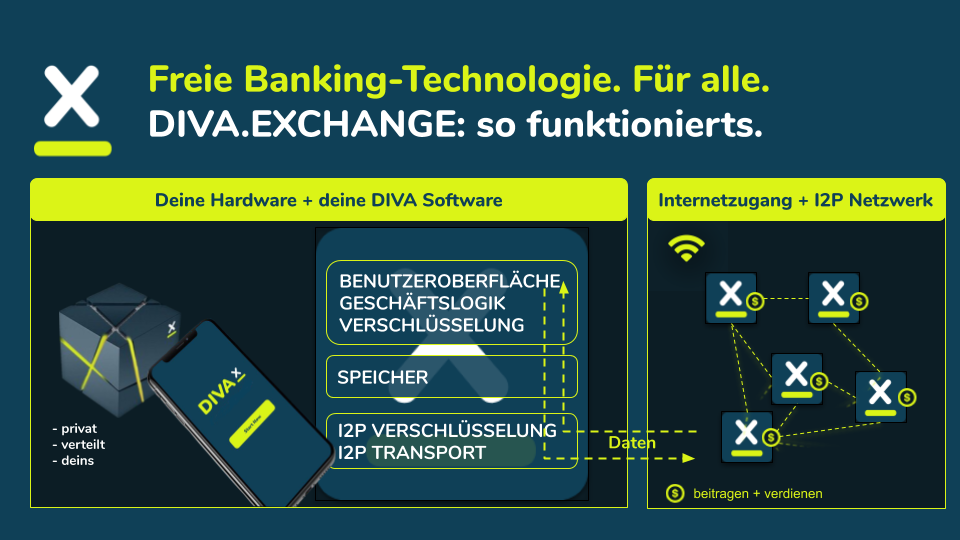
\includegraphics[width=1.0\textwidth]{img/divax-overview.png}
    \caption{Übersicht DIVA.EXCHANGE}\label{fig:divax_overview}
\end{figure}

Es besteht die Annahme, dass die Performanz des \glsname{i2p}-Netzwerk's nicht ausreichend ist, um für Endbenutzer schnell reagierende Applikationen auf dem Netzwerk anbieten zu können.
Das Netzwerk ist verglichen mit dem \glsname{tor}-Netzwerk klein und es können grössere Latenzen entstehen, um Anonymität für die Teilnehmer zu bieten.
Kurz vor Beginn dieser Arbeit dauerte das Hin- und Zurücksenden einer Nachricht durch das \glsname{i2p}-Netzwerk (Roundtrip) etwa drei bis acht Sekunden.

\begin{itemize}
    \item Eine Nachricht wird über mehrere Hops versendet und wird mehrmals weitergeleitet bevor diese bei ihrem Ziel ankommt.
    \item Fallen Hops aus müssen die Nachrichten neu über eine andere Route übermittelt werden.
    \item Jede Nachricht ist mehrfach verschlüsselt und jeder Knoten muss jeweils eine Verschlüsselungsschicht beim weiterleiten einer Nachricht entfernen was viele CPU-Zyklen kostet.
\end{itemize}

Im Rahmen dieser Arbeit soll folgende Problemstellung erarbeitet werden:

\begin{hyp}[H\ref{hyp:first}] \label{hyp:first}
    Ist eine steigende Anzahl von I2P-Knoten für die I2P-Netzwerk-Latenz (tiefer) vorteilhaft?
    Können Nachrichten schneller vom Sender zum Empfänger gelangen je mehr Knoten das I2P-Netzwerk hat?
\end{hyp}

Damit Applikationen auf dem I2P-Netzwerk gut funktionieren, soll ermittelt werden wie die Performance
verbessert werden soll.
Siehe auch die komplette Aufgabenstellung, die im Anhang~\fullref{ch:aufgabenstellung} zu finden ist.


\section{Ziel und Vision}\label{sec:ziel}

Ziel ist es aufzuzeigen unter welchen Umständen und Rahmenbedingungen Anwendungen auf dem \glsname{i2p}-Netzwerk kürzere Latenzzeiten aufweisen
und somit für Endbenutzer schneller reagieren können. Das Niveau an Anonymität soll aber zum Schutz der Privatsphäre nicht eingeschränkt werden.
Wird festgestellt, dass mehr Knoten in einem I2P-Netzwerk die Latenz verringert.
Diese Erkenntnis könnte auch unter Umständen mehr Personen dazu bewegen selber \glsname{i2p}-Knoten zu betreiben.
Dies wiederum würde das Netzwerk stärken und diverse Netzwerkeffekte könnten auftreten.
Zum Beispiel könnte dies dazu führen, das mehr Entwickler Applikationen für das Netzwerk erstellen und es auch aus Benutzerseite attraktiver wird.

% Welche Ziele, Fragestellungen werden mit dem Projekt verfolgt? Die Bedeutung, Auswirkung und
% Relevanz dieses Projektes für die unterschiedlichen Beteiligten soll aufgeführt werden.
% Typischerweise wird hier ein Verweis auf die Aufgabenstellung im Anhang gemacht.
